\documentclass[10pt]{article}
\usepackage[margin=1in]{geometry}
\usepackage{booktabs,graphicx}
\usepackage[hidelinks]{hyperref}
\title{What Survives a Compressed Handoff?\protect\\A Paired Study of One-Turn Multimodal Advice}
\author{Stan Chen}
\date{November 2026}
\begin{document}
\maketitle
\begin{abstract}
A coding agent can send a shorter record to a stronger advisor while retaining responsibility for the delivered artifact. Compression may remove a requirement or add overhead to an already short task. We compare a complete checkpoint, an executor-written summary, and a structured scoped packet on matched programming, chart-reading, and transcription tasks. Each arm receives the same task, original media, decision point, and one advice opportunity. We evaluate the final file against independent reference checks. This evidence draft accompanies the frozen data for subsequent manuscript preparation.
\end{abstract}

\section{Question and design}
We test whether the lower confidence bound for verified delivery with a scoped packet exceeds a prespecified margin of minus five percentage points relative to the complete checkpoint. A secondary comparison asks how much the packet format contributes under a common character limit. The full record contains the actual public brief and recorded local observations. The same original media are available in all three conditions. The final executor sees its checkpoint and usable advice and produces a file. Failed consultations, timeouts, and missing submissions remain in their assignment denominators.

The programming tasks come from the sanitized MBPP test set \cite{mbpp}, the images from ChartQA \cite{chartqa}, and the English recordings from FLEURS \cite{fleurs}. One independent source item contributes a single task. Three adjacent task conditions share an executor, advisor route, and deadline. Blind grading uses the original coding assertions, reference chart answers and reference transcripts. We normalize punctuation and case before scoring transcription. Pilot runs and product acceptance runs are retained separately.

\section{Verified delivery}
Confirmation included 180 independent tasks. The paired scoped-minus-full difference was +1.7 percentage points with a one-sided 95\% lower confidence bound of -2.2 points. The prespecified quality criterion was met. The all-modality cost ratio is unidentifiable from these receipts and rate cards. The descriptive scoped-minus-summary difference was +0.0 points. The pilot-based design called for 552 tasks before the registered cap of 180 was applied.

\begin{center}\begin{tabular}{lrrrr}
\toprule
Task set & Tasks & Full record & Free summary & Scoped packet \\
\midrule
Programming & 60 & 55 & 55 & 55 \\
Chart reading & 60 & 30 & 34 & 30 \\
Speech & 60 & 51 & 50 & 54 \\
All tasks & 180 & 136 & 139 & 139 \\
\bottomrule
\end{tabular}
\end{center}
Entries are counts of delivered files passing the independent checks before the deadline. Equal modality strata define the target workload.

\begin{figure}[ht]
\centering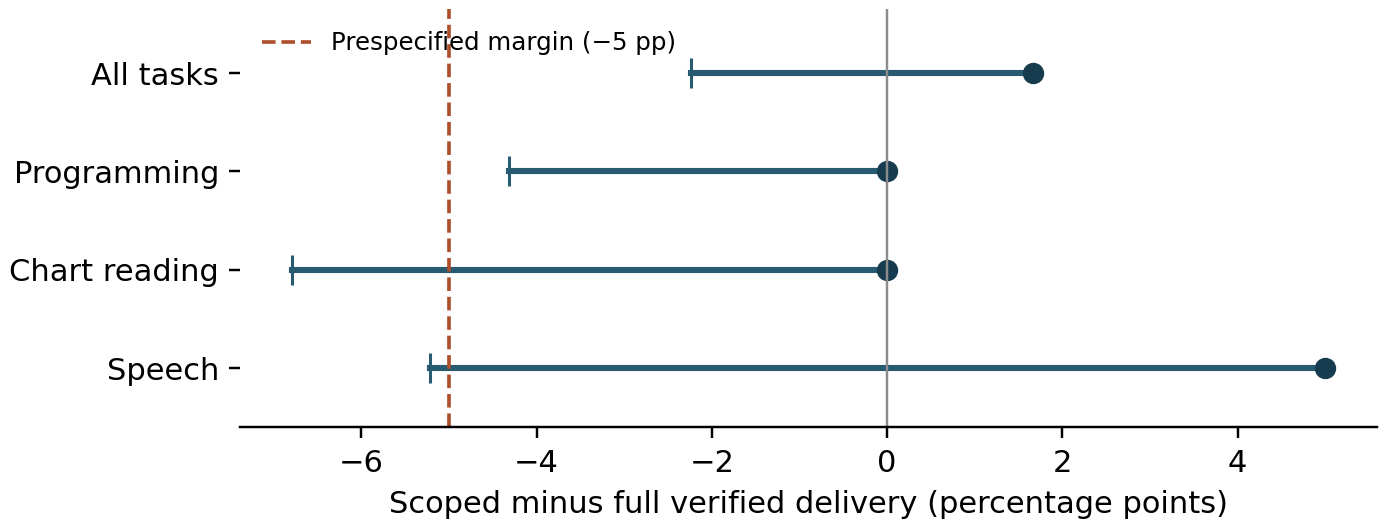
\includegraphics[width=.88\linewidth]{paired-quality.png}
\caption{Paired differences in verified delivery. Points are observed differences; the line extends to each one-sided 95\% lower score bound.}
\end{figure}

\section{Resource use and interpretation}
\begin{center}\small\begin{tabular}{lrrrr}
\toprule
Arm & Executor input & Advisor input & Median seconds & Priceable tasks \\
\midrule
Full record & 87,980 & 500,964 & 13.2 & 120/180 \\
Free summary & 158,407 & 435,197 & 18.6 & 120/180 \\
Scoped packet & 88,366 & 510,202 & 13.3 & 120/180 \\
\bottomrule
\end{tabular}
\end{center}
Input-token totals include only recorded amounts. The public archive gives coverage, output tokens, cache, elapsed time, and advisor statuses. A dollar comparison requires attributable rate and usage information for every required route. A lower advisor input count alone cannot establish a cheaper delivered result.

\section{Limitations and replication}
Short public tasks may have appeared in model training. Chart values and short English utterances capture only part of real multimodal use. Repeated speakers and shared chart conventions may reduce effective diversity. The full checkpoint in this study can already be shorter than the structured packet. Timing includes provider service conditions and concurrent execution. Native-host walkthroughs use automated testers approved by the project owner. They establish executable paths and provide no estimate of human onboarding time.

Model settings, source revisions, task and media digests, assignments, submitted outputs, and analysis scripts are included with the software release. No external arXiv submission is asserted by this package.

\begin{thebibliography}{9}
\bibitem{mbpp} J. Austin et al. Program Synthesis with Large Language Models. \url{https://arxiv.org/abs/2108.07732}.
\bibitem{chartqa} A. Masry et al. ChartQA: A Benchmark for Question Answering about Charts with Visual and Logical Reasoning. \url{https://aclanthology.org/2022.findings-acl.177/}.
\bibitem{fleurs} A. Conneau et al. FLEURS: Few-shot Learning Evaluation of Universal Representations of Speech. \url{https://arxiv.org/abs/2205.12446}.
\end{thebibliography}
\end{document}
